\chapter{Results and Discussion}
\label{ch:results}

\section{Experimental Setup}
All results in this chapter were produced by the final trained model with the deterministic action
$a_i = \tanh(\mu_\theta(o_i))$ and no additional controller behind the network. The final evaluation uses the
seven benchmark scenarios with 20 held-out seeds each (seeds 100000--100019, never used for training or model
selection), i.e.\ 140 episodes of 24\,s with eight drones. The demonstrations in
Sections~\ref{sec:demo}--\ref{sec:disturbance} use held-out seed 100000; the three-dimensional renderings are
drawn from the recorded simulator states and the screenshots are taken from the running web flight laboratory
with the same configuration.

\section{Demonstration of the Final System}
\label{sec:demo}
Figure~\ref{fig:render_crossing} shows a complete \emph{follow, yield, recover} cycle for a lateral crossing
object. Before the object arrives the eight drones hold their grid slots while following the target (a). As the
object crosses the formation, the drones nearest to its path move out of the way, in three dimensions, while the
others keep their places (b). After the object has passed, every drone returns to its own slot; the dotted
trails show the avoidance manoeuvre and the transparent sphere marks the earlier object position (c). In this
episode the minimum surface clearance was 0.298\,m and the formation was recovered 1.51\,s after the object
left the scene.

\begin{figure}[htbp]
  \centering
  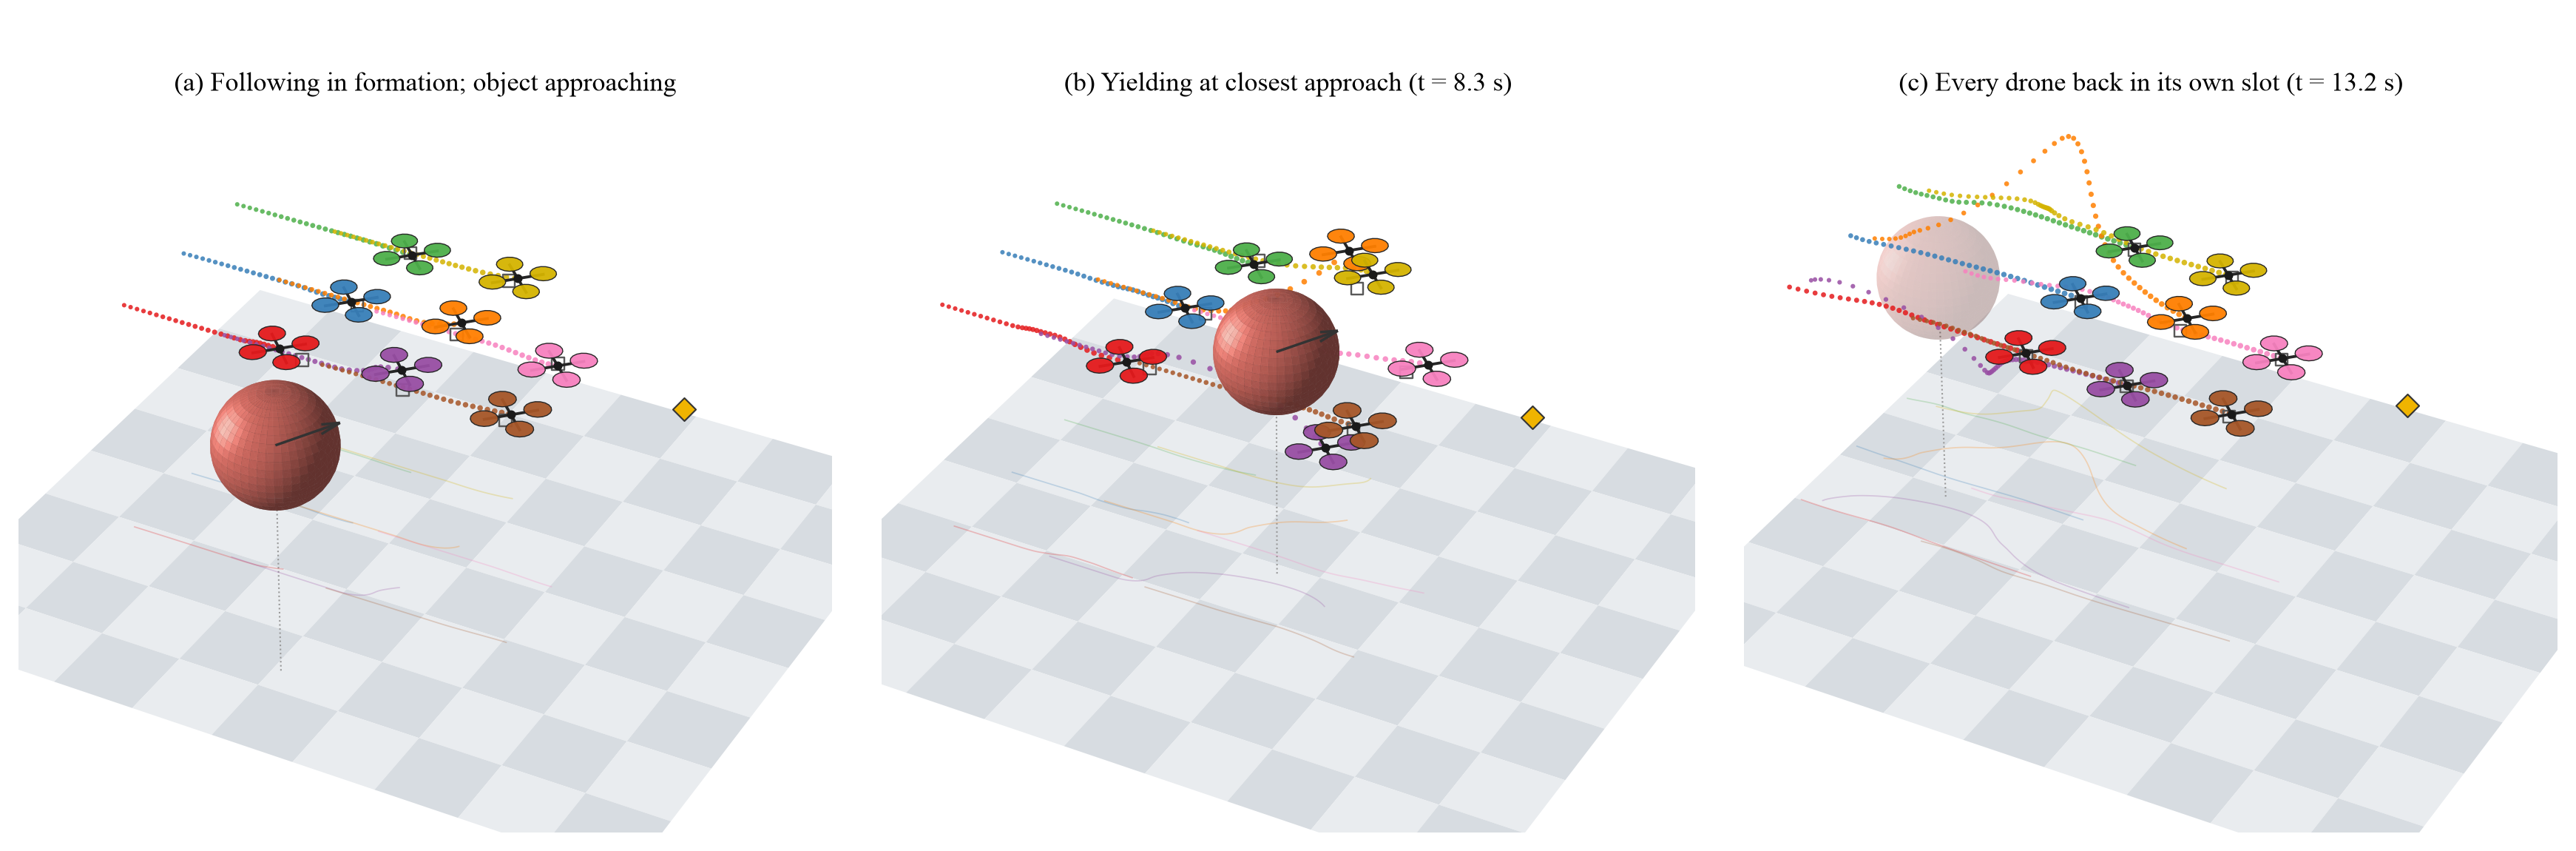
\includegraphics[width=0.95\textwidth]{fig_render_crossing}
  \caption[Follow, yield and recover behaviour of the final model]{Follow, yield and recover behaviour of the
  final model for a lateral crossing object (held-out seed 100000). Coloured quadrotors are the eight drones,
  dotted lines their trails, squares their assigned slots and the diamond the reference target.}
  \label{fig:render_crossing}
\end{figure}

The same episode in the web flight laboratory is shown in Figure~\ref{fig:viewer_sequence}. The live metrics
of the viewer agree with the offline evaluation, confirming that the demonstration is produced by the trained
network itself.

\begin{figure}[htbp]
  \centering
  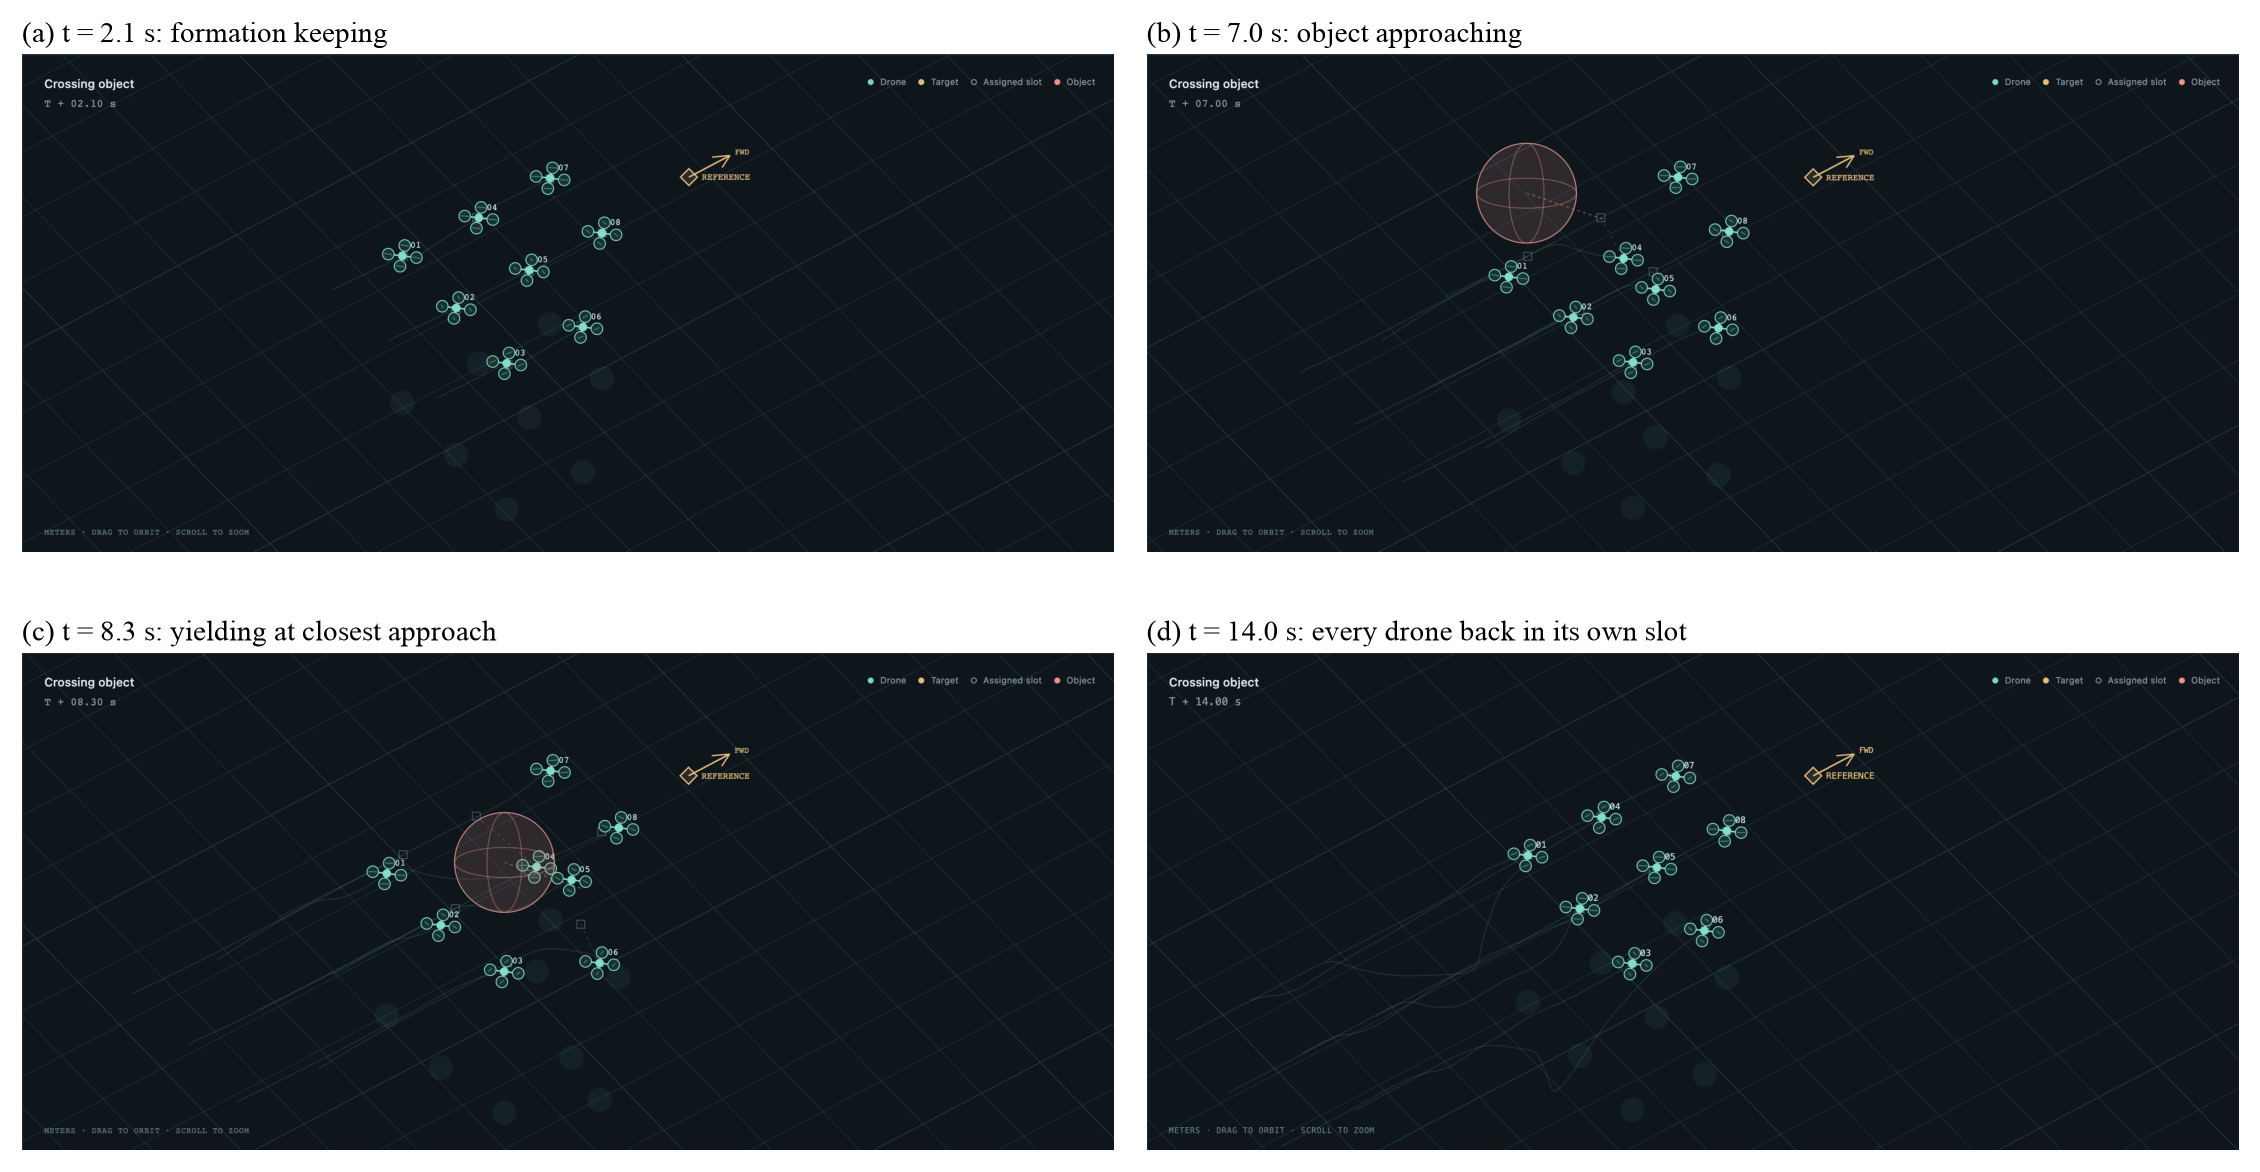
\includegraphics[width=0.76\textwidth]{fig_viewer_crossing_sequence}
  \caption[Crossing episode in the web flight laboratory]{The crossing episode of
  Figure~\ref{fig:render_crossing} in the SwarmFlow web flight laboratory: formation keeping (a), object
  approaching (b), yielding at closest approach (c) and complete recovery to the assigned slots (d).}
  \label{fig:viewer_sequence}
\end{figure}

Figure~\ref{fig:render_headon} shows the two more demanding disturbances. For a head-on object, which
approaches faster (relative speed 1.8--2.2\,m/s) and is larger, the formation opens around the object and
closes again, recovering 1.67\,s after the object left (a, b). In the repeated-crossing scenario a second
object arrives from the opposite side; the swarm yields again and recovers both disturbances, 1.51\,s and
2.00\,s after the respective exits (c).

\begin{figure}[htbp]
  \centering
  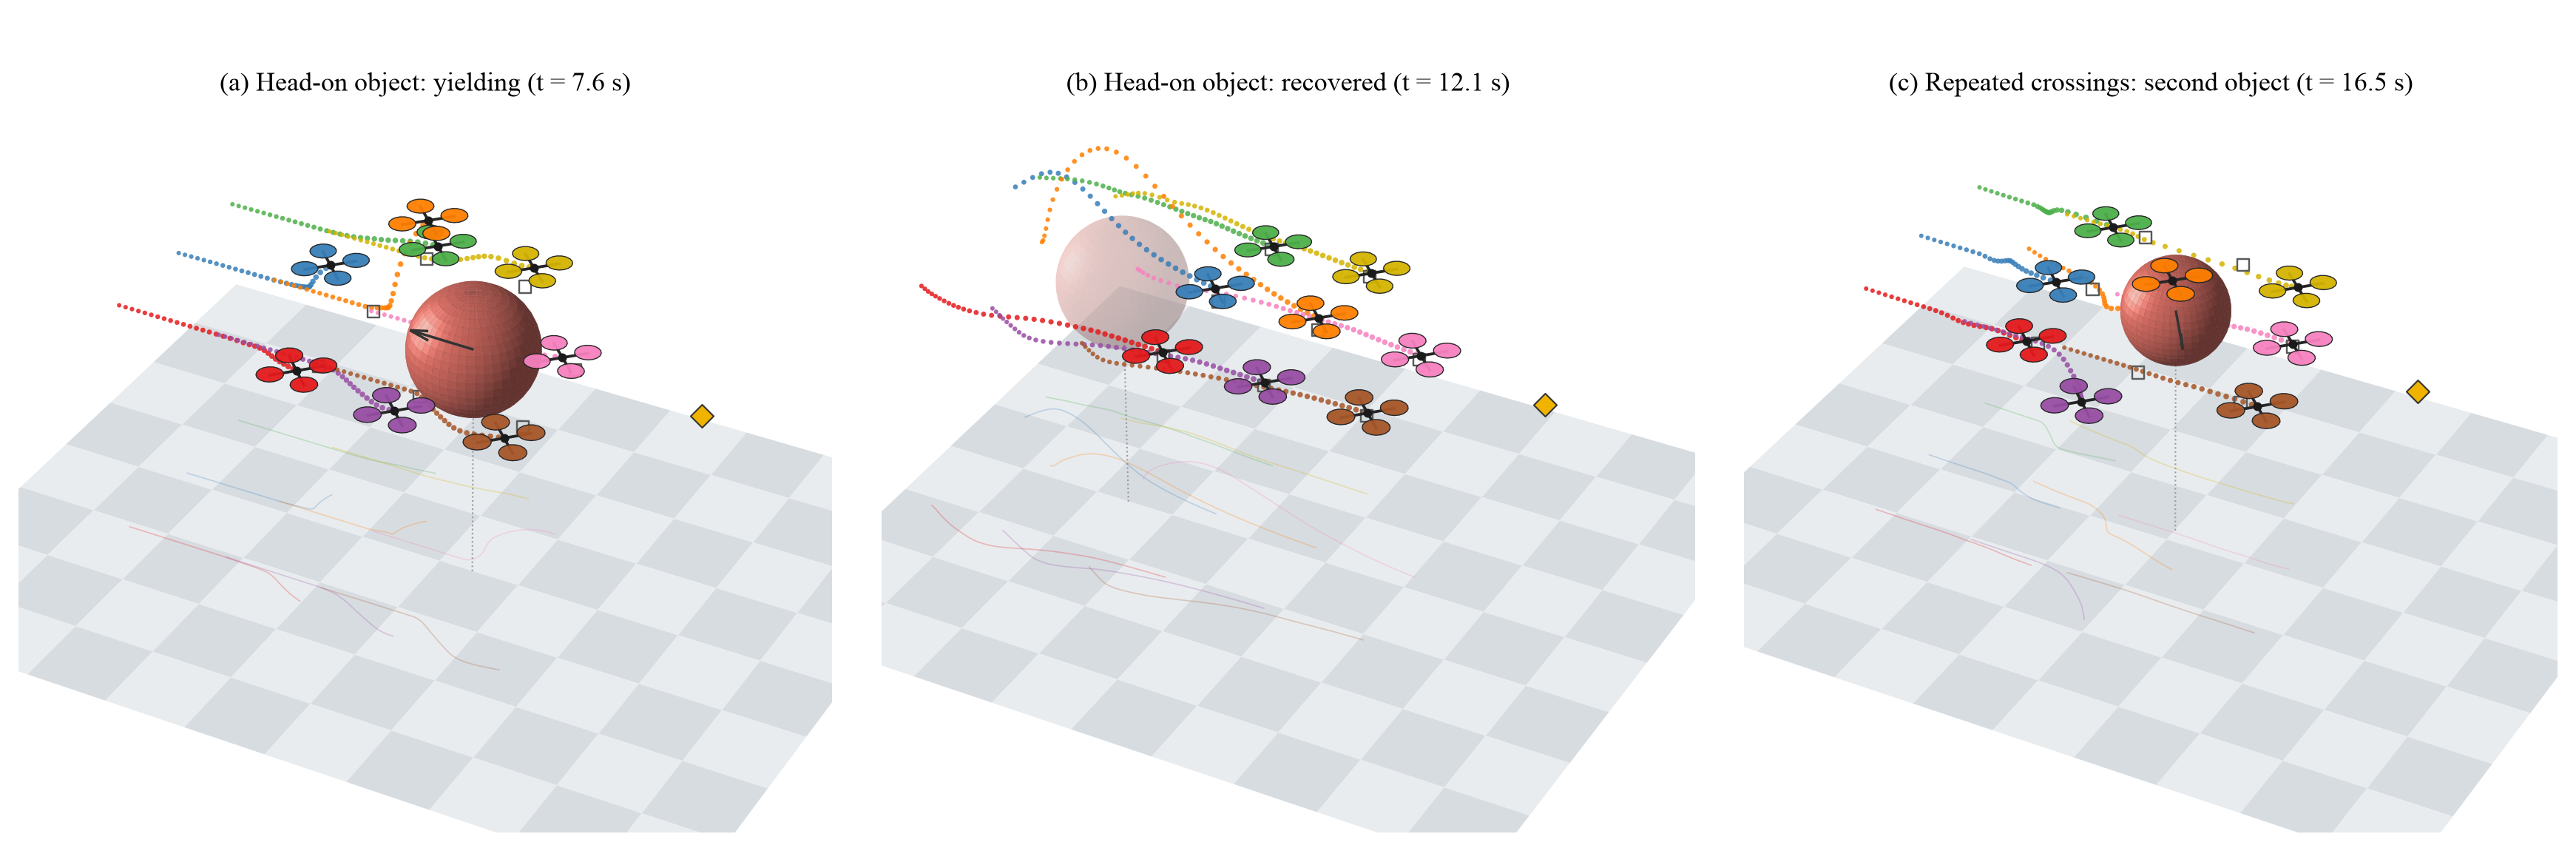
\includegraphics[width=0.95\textwidth]{fig_render_headon_double}
  \caption[Head-on and repeated-crossing behaviour]{Head-on object during yielding (a) and after recovery (b),
  and the second object of a repeated-crossing episode (c); held-out seed 100000.}
  \label{fig:render_headon}
\end{figure}

\section{Formation Disturbance and Recovery}
\label{sec:disturbance}
Figure~\ref{fig:timeseries} plots the distance of every drone to its own slot over time for the three disturbance
scenarios. Before the object arrives the error of all drones is only a few centimetres. During the object's
passage (shaded) only the drones close to its path deviate, by up to about 1.8\,m, and the swarm-level RMS error
returns below the 0.35\,m tolerance shortly after the object leaves. The green dashed lines mark the confirmed
recoveries; after recovery the formation error returns to its undisturbed level.

\begin{figure}[htbp]
  \centering
  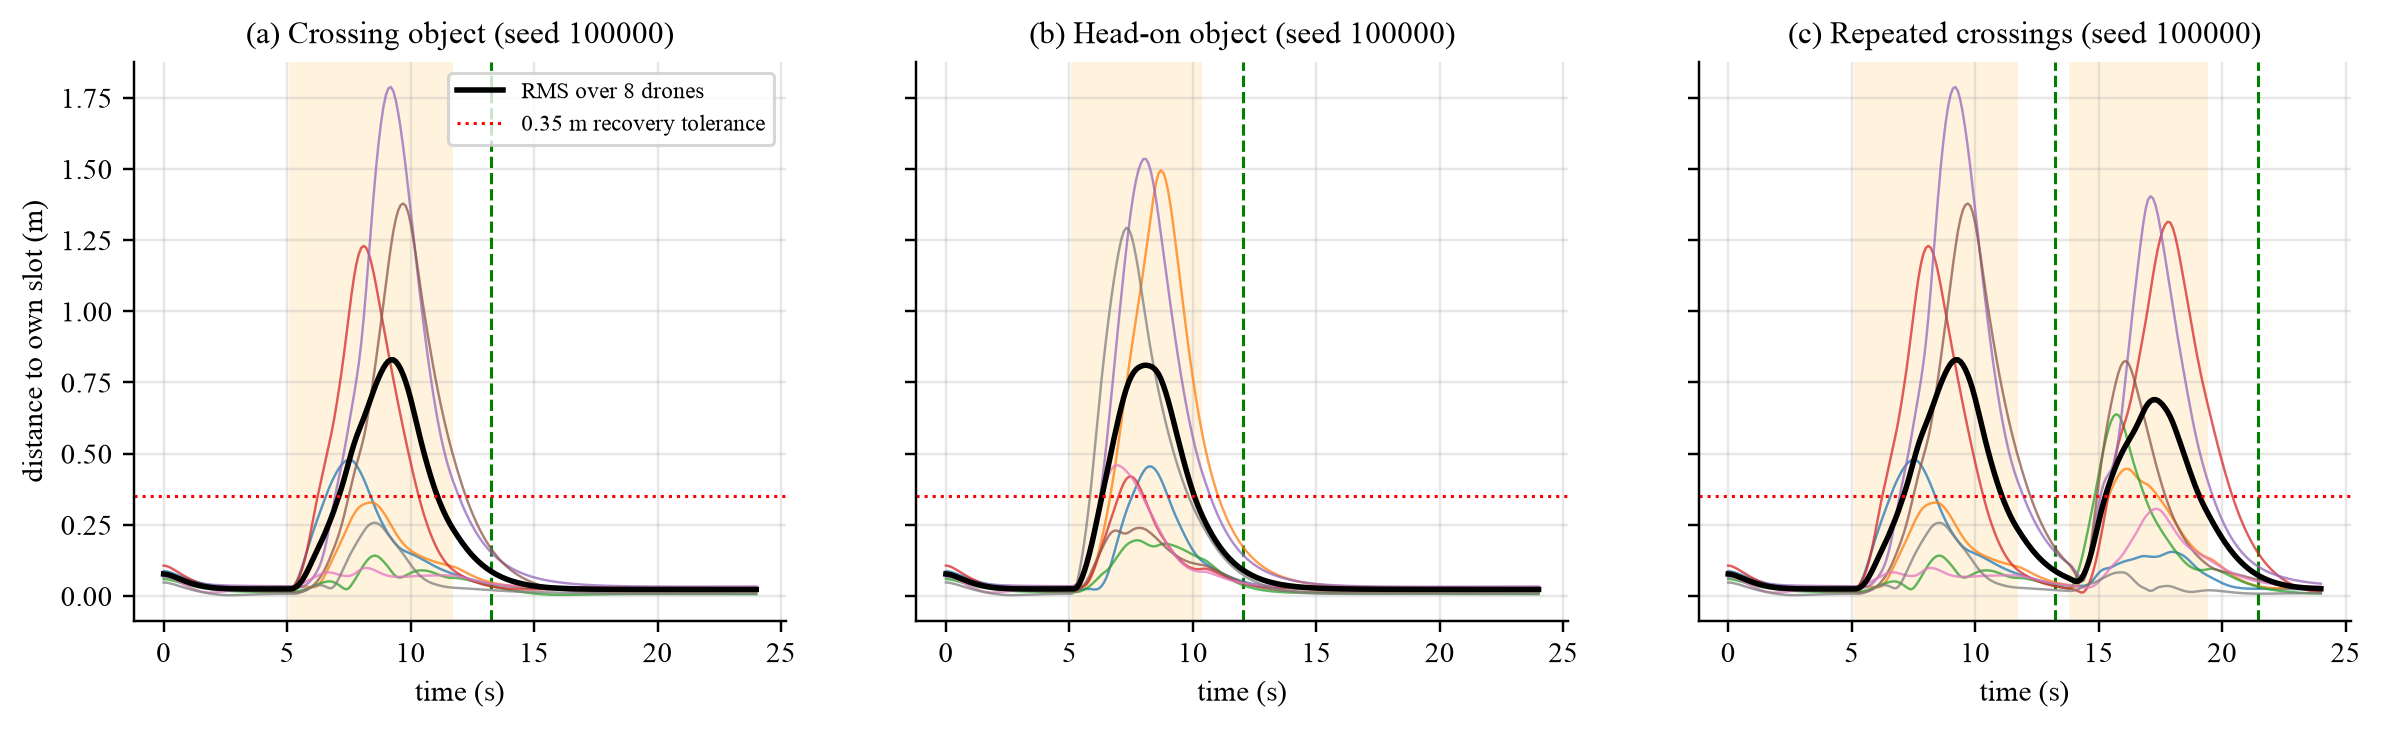
\includegraphics[width=0.9\textwidth]{fig_slot_error_timeseries}
  \caption[Distance of each drone to its own slot over time]{Distance of each drone to its own slot (thin
  lines) and RMS over the swarm (black) for held-out seed 100000. Shaded: object inside the scene; green dashed:
  confirmed recovery; red dotted: 0.35\,m recovery tolerance.}
  \label{fig:timeseries}
\end{figure}

\section{Held-Out Evaluation}
Table~\ref{tab:results} and Figure~\ref{fig:results} summarise the evaluation on the 140 held-out episodes.
The model completed 138 episodes (98.6\%) without failure and achieved 100\% success in six of the seven
scenarios. In the three undisturbed scenarios the formation error was 0.023\,m, 0.027\,m and 0.045\,m, well
below the 0.35\,m criterion; the wind gust increased it only to 0.176\,m. All 78 disturbances in the completed
episodes were recovered, 70 of all 80 within 5\,s; the mean recovery time was 1.9\,s for crossing and 2.4\,s for
head-on objects. In the head-on scenario 18 of 20 episodes were completed; in the remaining two, a drone made brief
contact with the object while passing it (minimum clearance $-0.04$\,m), which identifies the
head-on case as the main target for the further improvements described in Section~\ref{sec:future}.
Measured against the three criteria of Section~\ref{sec:problem}, the formation-precision criterion is met in every
undisturbed scenario, 98.6\% of the episodes are collision-free, and 87.5\% of the disturbances are recovered
within 5\,s; the remaining cases are concentrated in the head-on and double-crossing scenarios.

\begin{table}[htbp]
\centering
\caption{Held-out evaluation of the final model (20 unseen seeds per scenario)}
\label{tab:results}
\small
\begin{tabular}{@{}lccccc@{}}
\toprule
Scenario & Episodes & Slot RMSE & Disturbances & Mean / max & Min.\ surface\\
 & completed & (m) & recovered & recovery (s) & clearance (m)\\
\midrule
Hold             & 20/20 & 0.023 & -- & -- & 0.764\\
Follow           & 20/20 & 0.027 & -- & -- & 0.764\\
Turning target   & 20/20 & 0.045 & -- & -- & 0.764\\
Wind gust        & 20/20 & 0.176 & -- & -- & 0.764\\
Crossing         & 20/20 & 0.274 & 20/20 & 1.88 / 3.07 & 0.183\\
Head-on          & 18/20 & 0.289 & 18/20 & 2.43 / 4.12 & $-0.041$\\
Double crossing  & 20/20 & 0.393 & 40/40 & 3.47 / 11.36 & 0.009\\
\midrule
Total            & 138/140 & -- & 78/80 & -- & --\\
\bottomrule
\end{tabular}
\end{table}

\begin{figure}[htbp]
  \centering
  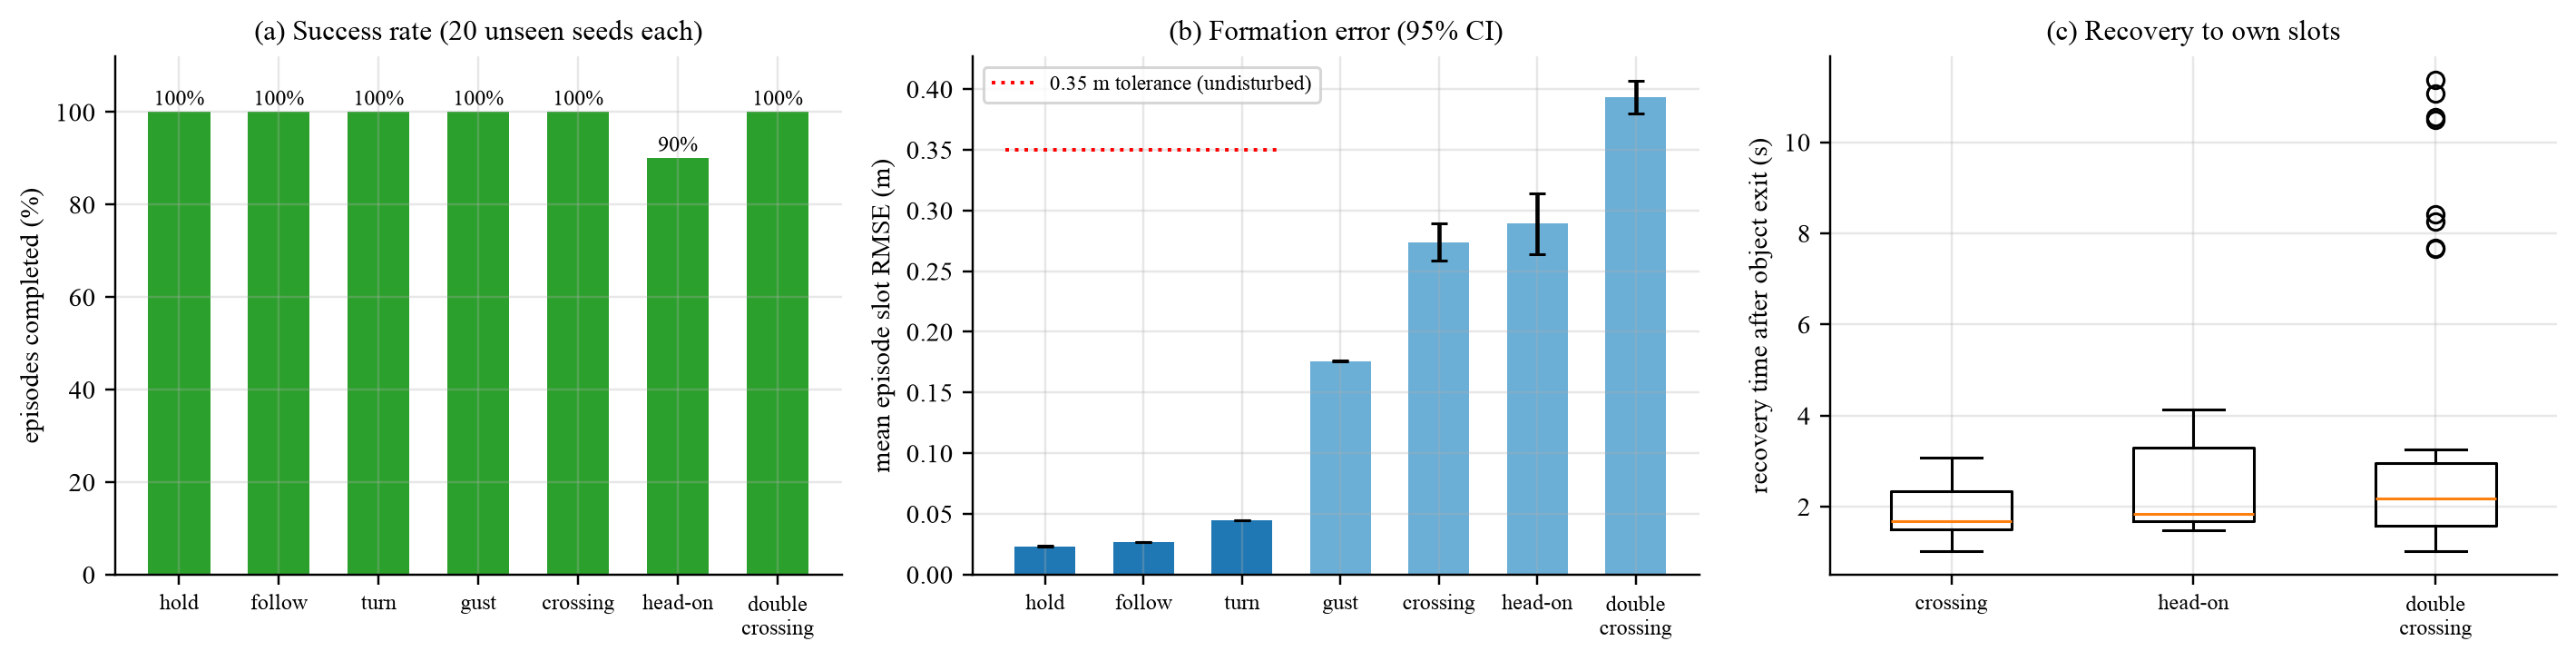
\includegraphics[width=0.9\textwidth]{fig_results_scenarios}
  \caption[Held-out success rate, formation error and recovery time]{Held-out evaluation of the final model:
  (a) episodes completed without failure, (b) mean episode slot RMSE with 95\% confidence intervals, and
  (c) recovery time after each object exit.}
  \label{fig:results}
\end{figure}

In the double-crossing scenario the second object sometimes enters while the swarm is still settling from the
first; the recovery clock of the first event then includes the second passage, which explains the few longer
recovery times in Figure~\ref{fig:results}(c).

\section{Training Behaviour}
Figure~\ref{fig:imitation}(a) shows the imitation error after each of the four demonstration rounds of every
stage: the action error decreases steadily (in stage~1 from $1.6\times10^{-3}$ to $4.0\times10^{-4}$) as DAgger
adds the states visited by the learner itself. During stage-1 PPO the formation error of the training episodes
fell from about 0.21\,m to below 0.06\,m (b), without a single training failure.

\begin{figure}[htbp]
  \centering
  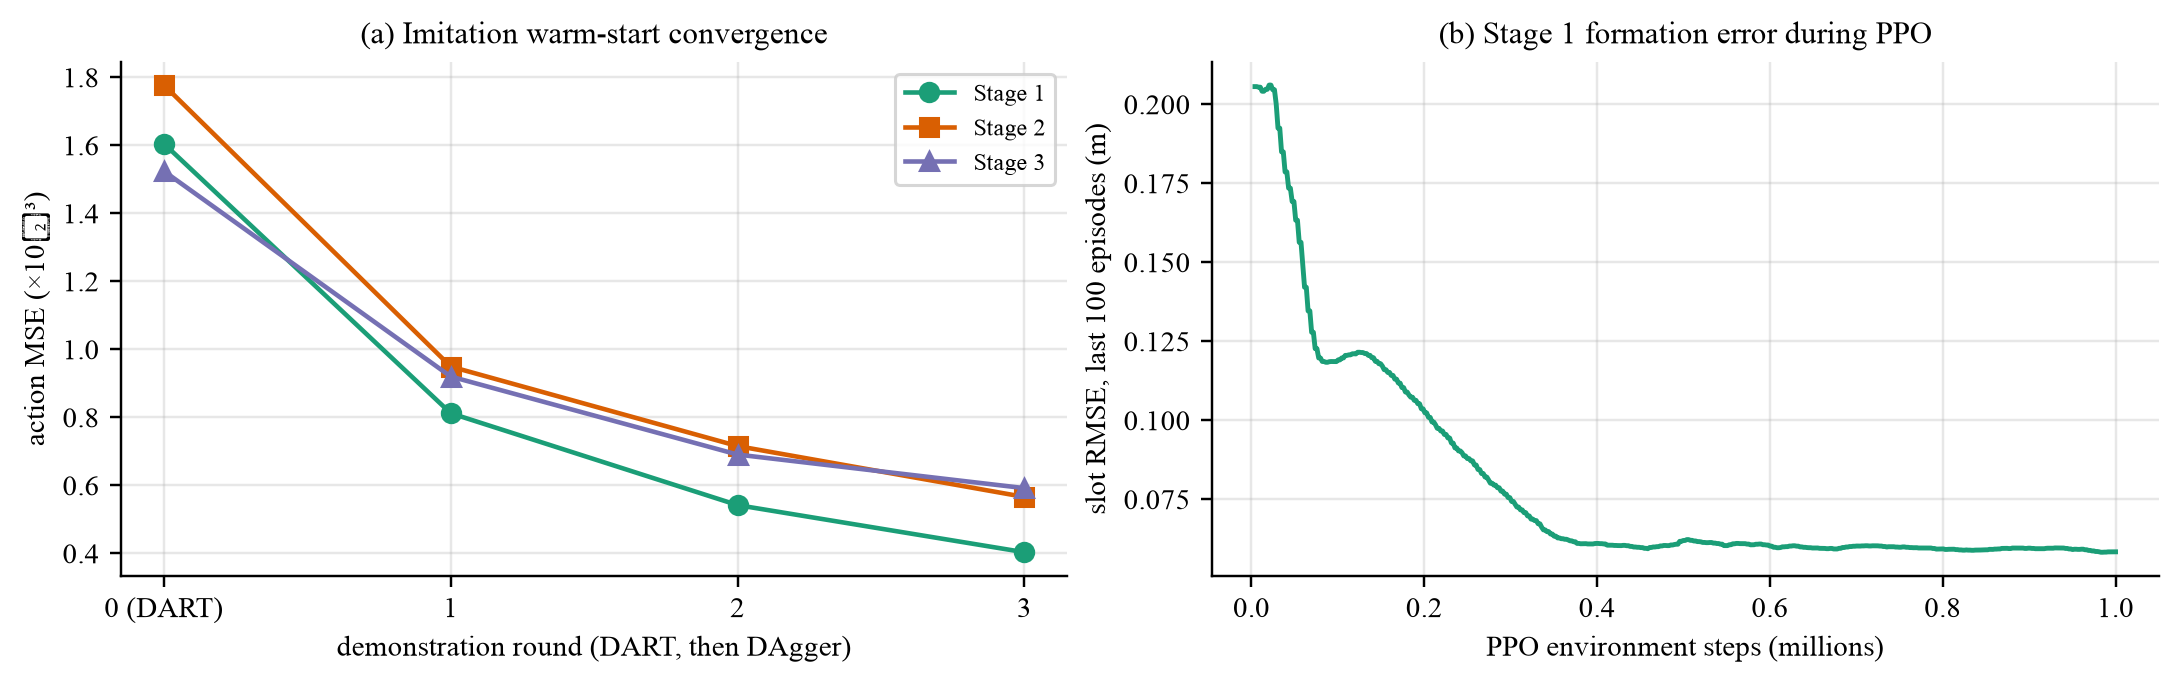
\includegraphics[width=0.85\textwidth]{fig_imitation_and_stage1}
  \caption[Imitation convergence and stage-1 training error]{(a) Action MSE after each demonstration round of
  the three stages. (b) Slot RMSE of the last 100 training episodes during stage-1 PPO.}
  \label{fig:imitation}
\end{figure}

Figure~\ref{fig:training_panel} shows the full
training history as reported by the web flight laboratory. The validation score stays close to 1.0 in stage~1;
in stages~2 and~3 the harder scenarios make the score vary between validations, and model selection retains
the best checkpoint of each stage (validation scores 0.997, 0.968 and 0.957). The selected final model reached
a held-out score of 0.936 on the unseen test seeds, close to its validation score, which indicates that it
generalises to new scenario instances.

\begin{figure}[htbp]
  \centering
  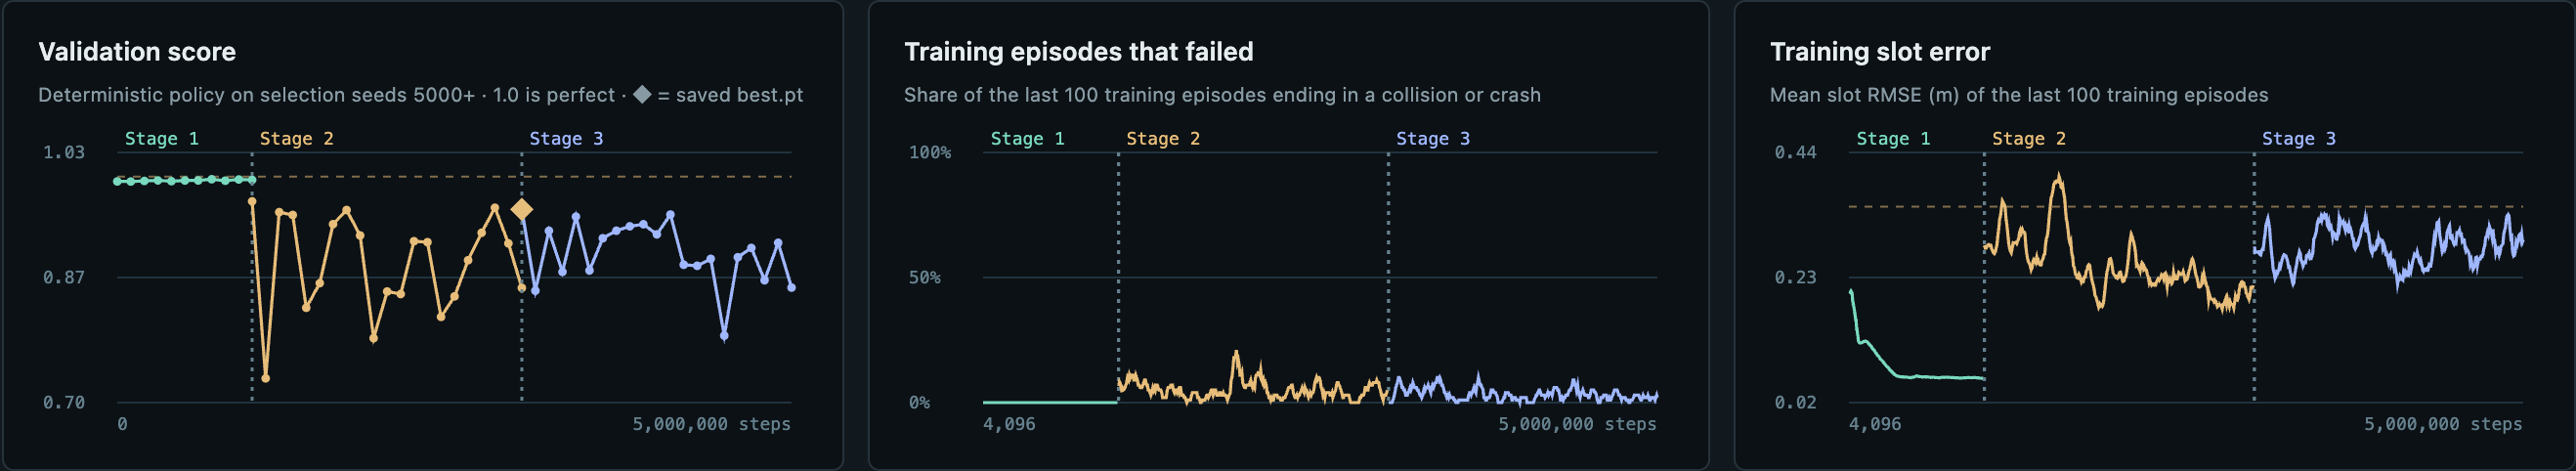
\includegraphics[width=0.9\textwidth]{viewer/model_training_charts}
  \caption[Training history of the final model in the flight laboratory]{Training history of the final model
  over the three-stage curriculum as displayed by the web flight laboratory: validation score (diamond: selected
  checkpoint), share of failed training episodes and training slot error.}
  \label{fig:training_panel}
\end{figure}

\section{Ongoing Development}
After the final model had been validated, a revised training configuration (version~4) was prepared. It enlarges
the clearance margins of the expert planner in the demonstration data (0.7\,m / 0.3\,m), refines the recovery
measurement when two disturbances overlap, and shortens the fine-tuning budget of stages~2 and~3 to 1\,M PPO
steps. This version was trained on a separate team machine: its first stage completed with a validation score
of 0.996, but errors were observed in the output during the subsequent training phase and the run was not
completed. The model presented in this report (version~3) therefore remains the final validated system, and the
completion of the version-4 training is part of the future work.

\section{Task, Achievement and Possible Beneficiaries}
The task of this project was to learn a decentralised controller that lets a drone swarm follow a target, yield
to moving objects and recover its formation. The achieved system meets the formation-precision criterion in all
undisturbed scenarios, completes 98.6\% of the held-out episodes without failure, returns every drone to its own
slot after every disturbance in the completed episodes, and runs as an interactive demonstration in which new
objects can be injected during flight. The approach and software can benefit:
\begin{itemize}
  \item researchers in multi-agent reinforcement learning and swarm robotics, as a compact and reproducible
        benchmark with explicit recovery metrics;
  \item developers of drone-show, inspection and surveillance systems that require formation flight in shared
        airspace;
  \item educators, through the interactive flight laboratory that visualises learned multi-agent behaviour.
\end{itemize}

\section{Review of Contributions}
\begin{enumerate}
  \item A PettingZoo multi-agent environment for formation following, yielding and same-slot recovery with a
        stabilised flight model and continuous swept collision detection.
  \item A bounded, per-drone reward with culprit-only failure penalties and a quantitative recovery criterion.
  \item A shared, permutation-invariant actor--critic network with masked multi-head attention pooling over
        neighbours and objects.
  \item A three-stage curriculum combining DART and DAgger initialisation from an expert planner with PPO and
        GAE fine-tuning, collision-state replay and validation-based model selection.
  \item A held-out evaluation protocol with disjoint seed ranges and 40 automated unit tests.
  \item An interactive web flight laboratory for live demonstration, object injection and training inspection.
\end{enumerate}

\section{Scope for Future Work}
\label{sec:future}
\begin{itemize}
  \item Complete the version-4 training and train several random seeds to quantify run-to-run variation.
  \item Increase the clearance of the head-on manoeuvre, for example by larger demonstration margins or a
        predictive safety layer evaluated as a separate controller.
  \item Evaluate generalisation to 4, 12 and 16 drones, other formation geometries, noisy and dropped
        observations, and the dense-obstacle and terrain worlds already available in the viewer.
  \item Replay the scenarios in a full rigid-body quadrotor simulator such as gym-pybullet-drones
        \cite{panerati2021learning} and study transfer to real hardware.
  \item Compare the local critic with a centralised critic \cite{yu2022surprising} and add recurrent memory for
        partially observed situations.
\end{itemize}
